% ==============================================================
%  Design of an I3C Communication Controller — Graduation Thesis
%  Vo Minh Huy (22207042), HCMUS, May 2026
% ==============================================================
\documentclass[12pt, a4paper, oneside]{report}

% ── Encoding & fonts ──────────────────────────────────────────
\usepackage[T1]{fontenc}
\usepackage[utf8]{inputenc}
\usepackage{lmodern}
\usepackage{microtype}

% ── Page geometry ─────────────────────────────────────────────
\usepackage[
  top=25mm, bottom=25mm,
  left=35mm, right=20mm,
  headheight=15pt
]{geometry}

% ── Line spacing ──────────────────────────────────────────────
\usepackage{setspace}
\onehalfspacing

% ── Headers / footers ─────────────────────────────────────────
\usepackage{fancyhdr}
\pagestyle{fancy}
\fancyhf{}
\fancyhead[R]{\small\leftmark}
\fancyfoot[C]{\thepage}
\renewcommand{\headrulewidth}{0.4pt}

% ── Chapter titles ────────────────────────────────────────────
\usepackage{titlesec}
\titleformat{\chapter}[block]
  {\normalfont\Large\bfseries}{Chapter \thechapter.}{1em}{}
\titlespacing*{\chapter}{0pt}{20pt}{15pt}

% ── Tables ────────────────────────────────────────────────────
\usepackage{booktabs}
\usepackage{longtable}
\usepackage{array}
\usepackage{multirow}
\usepackage{tabularx}
\newcolumntype{L}[1]{>{\raggedright\arraybackslash}p{#1}}
\newcolumntype{C}[1]{>{\centering\arraybackslash}p{#1}}

% ── Graphics ──────────────────────────────────────────────────
\usepackage{graphicx}
\usepackage{float}
\usepackage{tikz}
\usetikzlibrary{shapes.geometric, arrows.meta, positioning, fit, calc}

% ── Code listings ─────────────────────────────────────────────
\usepackage{listings}
\usepackage{xcolor}

\definecolor{codegreen}{rgb}{0,0.5,0}
\definecolor{codegray}{rgb}{0.4,0.4,0.4}
\definecolor{codepurple}{rgb}{0.5,0,0.5}
\definecolor{codeblue}{rgb}{0,0,0.7}
\definecolor{backgray}{rgb}{0.96,0.96,0.96}

\lstdefinelanguage{SystemVerilog}{
  morekeywords={module, endmodule, input, output, inout, logic, wire, reg,
    always_ff, always_comb, always, posedge, negedge, if, else, case,
    endcase, begin, end, assign, parameter, localparam, typedef, struct,
    packed, enum, typedef, import, package, endpackage, function,
    endfunction, initial, for, while, repeat, fork, join, interface,
    endinterface, modport, clocking, endclocking, assert, property,
    sequence, default, generate, endgenerate, genvar, integer, bit,
    byte, int, unsigned, signed, void, string, automatic, static},
  sensitive=true,
  morecomment=[l]{//},
  morecomment=[s]{/*}{*/},
  morestring=[b]",
}

\lstset{
  language=SystemVerilog,
  backgroundcolor=\color{backgray},
  basicstyle=\ttfamily\small,
  keywordstyle=\color{codeblue}\bfseries,
  commentstyle=\color{codegreen}\itshape,
  stringstyle=\color{codepurple},
  numberstyle=\tiny\color{codegray},
  numbers=left,
  stepnumber=1,
  numbersep=8pt,
  showspaces=false,
  showstringspaces=false,
  showtabs=false,
  frame=single,
  framerule=0.4pt,
  rulecolor=\color{codegray},
  breaklines=true,
  breakatwhitespace=false,
  tabsize=2,
  captionpos=b,
  xleftmargin=15pt,
  xrightmargin=5pt,
}

% plain text / shell listing
\lstdefinestyle{plain}{
  language={},
  basicstyle=\ttfamily\small,
  backgroundcolor=\color{backgray},
  frame=single,
  framerule=0.4pt,
  rulecolor=\color{codegray},
  numbers=none,
  breaklines=true,
}

% ── Hyperlinks ────────────────────────────────────────────────
\usepackage[
  colorlinks=true,
  linkcolor=black,
  citecolor=black,
  urlcolor=black,
  bookmarks=true,
  pdfauthor={Vo Minh Huy},
  pdftitle={Design of an I3C Communication Controller},
]{hyperref}

% ── Misc utilities ────────────────────────────────────────────
\usepackage{enumitem}
\usepackage{amsmath}
\usepackage{caption}
\usepackage{subcaption}
\usepackage{pdfpages}
\usepackage{tocloft}
\usepackage{emptypage}

% ── Custom commands ───────────────────────────────────────────
\newcommand{\signal}[1]{\texttt{#1}}
\newcommand{\reg}[1]{\texttt{#1}}
\newcommand{\file}[1]{\texttt{#1}}
\newcommand{\module}[1]{\texttt{#1}}
\newcommand{\state}[1]{\textsc{#1}}
\newcommand{\ie}{\textit{i.e.},\ }
\newcommand{\eg}{\textit{e.g.},\ }

% ── Bibliography ──────────────────────────────────────────────
\usepackage[numbers,sort&compress]{natbib}

% ==============================================================
\begin{document}

% ── Title Page ────────────────────────────────────────────────
\begin{titlepage}
\centering
\vspace*{1cm}

{\large\bfseries HO CHI MINH CITY UNIVERSITY OF SCIENCE\\
FACULTY OF ELECTRONICS AND TELECOMMUNICATIONS}

\vspace{0.5cm}
\rule{\linewidth}{0.5pt}

\vspace{2cm}
{\LARGE\bfseries Design of an I3C\\[0.3em] Communication Controller}

\vspace{0.5cm}
{\large Graduation Thesis}

\vspace{2cm}
\begin{tabular}{ll}
\textbf{Student:}    & Vo Minh Huy \\[4pt]
\textbf{Student ID:} & 22207042 \\[4pt]
\textbf{Class:}      & 22DVT\_CLC1 \\[4pt]
\textbf{Supervisor:} & Nguyen Duy Manh Thi \\[4pt]
\textbf{Credits:}    & 10 \\
\end{tabular}

\vfill
{\large Ho Chi Minh City, May 2026}
\end{titlepage}

% ── Front matter ──────────────────────────────────────────────
\pagenumbering{roman}

% ── Abstract ──────────────────────────────────────────────────
\chapter*{Abstract}
\addcontentsline{toc}{chapter}{Abstract}

This thesis presents the design and verification of a simplified MIPI I3C Basic v1.1.1
master controller implemented in SystemVerilog. The design operates in Single Data Rate
(SDR) mode at up to 12.5\,MHz, supports Dynamic Address Assignment (DAA) via the ENTDAA
protocol, performs private read/write transfers, and maintains I2C Fast Mode (400\,kHz)
backward compatibility. The controller is derived from the open-source CHIPS Alliance
\textit{i3c-core} reference implementation through a study-and-improve methodology,
achieving approximately 92\% code reduction --- from roughly 25\,000 to 4\,100 lines of
RTL --- while retaining full functional coverage of the specified feature set.

A UVM-based functional verification environment is developed alongside the RTL. A
systematic bug analysis identifies 22 issues across 18 source files, including 3 critical
defects, each with documented root-cause analysis and remediation. The resulting design
demonstrates the complete frontend IC design pipeline from specification study through RTL
implementation and functional verification.

\vspace{1.5em}
\noindent\textbf{Keywords:} I3C, MIPI, SystemVerilog, RTL design, SDR mode, ENTDAA, UVM,
functional verification, master controller, HCI queues.

% ── Table of Contents ─────────────────────────────────────────
\tableofcontents

% ── List of Figures / Tables ──────────────────────────────────
\listoffigures
\listoftables

% ── Main matter ───────────────────────────────────────────────
\cleardoublepage
\pagenumbering{arabic}

% ==============================================================
\chapter{Introduction}
% ==============================================================

\section{Motivation}

Modern System-on-Chip (SoC) and embedded system designs increasingly demand high-speed,
low-power serial communication capable of connecting many peripheral devices on a shared
two-wire bus. The Inter-Integrated Circuit (I2C) bus, while ubiquitous, has
well-documented limitations: a maximum speed of 1\,MHz (Fast-Mode Plus), static address
assignment that creates address conflicts, and open-drain signaling that wastes power
through continuous pull-up resistor current.

The MIPI Alliance introduced the I3C (Improved Inter-Integrated Circuit) bus standard to
address these deficiencies. I3C retains the two-wire topology and full I2C backward
compatibility while delivering a 12.5-fold increase in maximum clock frequency,
push-pull signaling for lower power, and a dynamic address assignment protocol that
eliminates static address conflicts.

The design of an I3C master controller provides a comprehensive exercise in the frontend
digital IC design pipeline: specification study, architectural decomposition, RTL
implementation in SystemVerilog, and functional verification using UVM. This pipeline
mirrors industry practice and is directly relevant to careers in integrated circuit
design and verification.

\section{Objectives}

This thesis aims to:
\begin{enumerate}
  \item Develop a thorough understanding of the MIPI I3C Basic v1.1.1 specification,
        with focus on SDR mode, the ENTDAA dynamic address assignment protocol, private
        read/write transactions, and I2C backward compatibility.
  \item Design an I3C master controller at the RTL level using SystemVerilog, derived
        from and improving upon the open-source CHIPS Alliance i3c-core reference
        implementation.
  \item Build a UVM-based functional verification environment to validate all specified
        transfer modes.
  \item Document design decisions, architectural improvements over the reference, and
        identified bugs with their remediation.
\end{enumerate}

\section{Scope}

\subsection*{In Scope}
\begin{itemize}
  \item SDR mode operation up to 12.5\,MHz
  \item Dynamic Address Assignment via ENTDAA
  \item Private write and read transfers (immediate and regular)
  \item I2C Fast Mode backward compatibility (400\,kHz, hardcoded timing)
  \item Essential Common Command Codes: ENTDAA (0x07), ENEC (0x00/0x80), DISEC (0x01/0x81)
  \item Master (Active Controller) role only
  \item RTL-level design; full physical implementation is out of scope
\end{itemize}

\subsection*{Explicitly Excluded}
\begin{itemize}
  \item In-Band Interrupts (IBI) and Hot-Join
  \item HDR modes (HDR-DDR, HDR-TSL, HDR-TSP)
  \item Multi-master / secondary controller operation
  \item Target (slave) mode
  \item Bus recovery protocol
  \item Full MIPI HCI compliance
\end{itemize}

\section{Methodology}

This thesis adopts a \textbf{study-and-improve} methodology. The starting point is the
CHIPS Alliance i3c-core reference implementation --- a production-grade I3C controller
designed for the Caliptra root-of-trust subsystem. The process follows four steps:

\begin{enumerate}
  \item \textbf{Study} --- analyze the reference design's architecture, module
        decomposition, FSM structures, and protocol handling.
  \item \textbf{Extract} --- identify the subset of modules and logic relevant to the
        basic master controller scope.
  \item \textbf{Simplify} --- eliminate complexity introduced by Caliptra-specific
        requirements (AXI adapters, target mode, IBI, auto-generated CSR).
  \item \textbf{Improve} --- complete unimplemented FSM states, fix known architectural
        issues, implement proper OD/PP switching, and write a clean hand-crafted
        register file.
\end{enumerate}

This approach grounds the design in a proven architecture while producing original
contributions in completion, simplification, and focused verification.

\section{Thesis Organization}

\begin{description}
  \item[Chapter 2] covers the MIPI I3C protocol: bus topology, SDR frame format, bus
        conditions, timing parameters, CCC commands, and the ENTDAA sequence.
  \item[Chapter 3] analyzes the CHIPS Alliance i3c-core reference and identifies reuse,
        simplification, and improvement opportunities.
  \item[Chapter 4] describes the proposed system architecture and module decomposition.
  \item[Chapter 5] documents the RTL implementation of each module.
  \item[Chapter 6] describes the UVM verification environment and test plan.
  \item[Chapter 7] presents the systematic bug analysis: 22 issues across 18 source files.
  \item[Chapter 8] discusses results and evaluates the design against objectives.
  \item[Chapter 9] concludes with a summary and future work directions.
\end{description}

% ==============================================================
\chapter{Background: MIPI I3C Protocol}
% ==============================================================

\section{Overview}

I3C (Improved Inter-Integrated Circuit) is a serial communication bus standard defined
by the MIPI Alliance. It is designed to unify sensor and actuator communication in
modern SoC designs, replacing I2C and SPI with a single, faster, lower-power interface
while preserving backward compatibility with existing I2C devices. The target
specification for this thesis is \textbf{MIPI I3C Basic v1.1.1 with Errata 01 (2022)}.

\section{Bus Topology}

I3C uses a shared two-wire bus: \textbf{SCL} (Serial Clock), driven exclusively by the
master in SDR mode, and \textbf{SDA} (Serial Data), which is bidirectional. Both lines
have an internal pull-up to VDD; unlike I2C, no external pull-up resistor is required
for I3C-native devices.

The bus supports two signaling modes:
\begin{itemize}
  \item \textbf{Open-drain}: used after START (address phase) and for all I2C legacy
        communication. Allows wired-AND arbitration between multiple drivers.
  \item \textbf{Push-pull}: used during I3C SDR data phases for maximum throughput
        (12.5\,MHz). Requires the controller to switch the PHY driver mode.
\end{itemize}

\section{I3C versus I2C}

Table~\ref{tab:i3c_vs_i2c} summarizes the key differences between I2C Fast-Mode Plus
and I3C SDR mode.

\begin{table}[H]
\centering
\caption{Comparison of I2C Fast-Mode Plus and I3C SDR}
\label{tab:i3c_vs_i2c}
\begin{tabularx}{\textwidth}{L{5cm} L{4.5cm} L{4.5cm}}
\toprule
\textbf{Feature} & \textbf{I2C (Fm+)} & \textbf{I3C (SDR)} \\
\midrule
Max clock frequency  & 1\,MHz         & 12.5\,MHz \\
Max data rate        & 1\,Mbit/s      & 12.5\,Mbit/s \\
Signaling            & Open-Drain only & OD + Push-Pull \\
Address space        & 7-bit, static  & 7-bit, dynamic \\
Address assignment   & Fixed / SW     & Dynamic (ENTDAA) \\
Clock stretching     & Yes (target)   & Not permitted (target) \\
Pull-up resistor     & External       & Internal \\
Backward compat.     & N/A            & Full I2C Fm+ \\
Error detection      & ACK/NACK       & Parity (T-bit) \\
\bottomrule
\end{tabularx}
\end{table}

\section{SDR Frame Format}

An I3C SDR transfer frame has the structure:

\begin{lstlisting}[style=plain, caption={I3C SDR frame format}]
[START] [Addr(7-bit) + RnW(1-bit) + T-bit] [Data(8-bit) + T-bit] ... [STOP]
\end{lstlisting}

Each byte is 9 bits: 8 data bits followed by a \textbf{T-bit} (Transition bit). The
T-bit semantics differ by phase:

\begin{itemize}
  \item \textbf{Address byte T-bit}: ACK/NACK from the target (0 = ACK, 1 = NACK).
  \item \textbf{Write data byte T-bit}: Odd parity over the 8 data bits, computed by
        the master and verified by the target.
  \item \textbf{Read data byte T-bit}: End-of-data indicator from the target (0 = last
        byte, 1 = more data to follow).
\end{itemize}

All transfers are MSB-first. The signaling mode transitions from open-drain (address
phase) to push-pull (data phase) after the repeated START.

\section{Bus Conditions}

\begin{table}[H]
\centering
\caption{I3C bus conditions}
\label{tab:bus_conditions}
\begin{tabular}{L{4cm} L{9cm}}
\toprule
\textbf{Condition} & \textbf{Definition} \\
\midrule
START (S)           & SDA falls while SCL is HIGH \\
REPEATED START (Sr) & START issued without a preceding STOP \\
STOP (P)            & SDA rises while SCL is HIGH \\
Bus Idle            & Both SCL and SDA HIGH; no active transfer \\
\bottomrule
\end{tabular}
\end{table}

\section{Timing Parameters}

The controller requires a system clock of at least \textbf{333\,MHz} to satisfy the
most demanding I3C timing constraint: $t_{\text{SCO,max}} = 12\,\text{ns}$ (clock-to-data
output). At 333\,MHz, four pipeline stages consume $4 \times 3\,\text{ns} = 12\,\text{ns}$.

\begin{table}[H]
\centering
\caption{I3C SDR timing defaults at 333\,MHz system clock}
\label{tab:timing}
\begin{tabular}{llrr}
\toprule
\textbf{Parameter} & \textbf{Symbol} & \textbf{Minimum} & \textbf{Cycles (333\,MHz)} \\
\midrule
SCL LOW period      & $t_{\text{LOW}}$    & 24\,ns & 8 \\
SCL HIGH period     & $t_{\text{HIGH}}$   & 24\,ns & 8 \\
Rise time           & $t_R$               & ---    & 4 \\
Fall time           & $t_F$               & ---    & 4 \\
START setup time    & $t_{\text{SU,STA}}$ & ---    & 8 \\
START hold time     & $t_{\text{HD,STA}}$ & ---    & 8 \\
STOP setup time     & $t_{\text{SU,STO}}$ & 12\,ns & 4 \\
\bottomrule
\end{tabular}
\end{table}

\section{Common Command Codes}

CCCs are issued using the reserved broadcast address \signal{7'h7E}. This thesis
implements only three essential CCCs, as shown in Table~\ref{tab:cccs}.

\begin{table}[H]
\centering
\caption{Implemented Common Command Codes}
\label{tab:cccs}
\begin{tabular}{ccll}
\toprule
\textbf{Code} & \textbf{Mnemonic} & \textbf{Type} & \textbf{Description} \\
\midrule
0x00 & ENEC   & Broadcast & Enable events on all targets \\
0x01 & DISEC  & Broadcast & Disable events on all targets \\
0x07 & ENTDAA & Broadcast & Enter Dynamic Address Assignment \\
0x80 & ENEC   & Direct    & Enable events (specific target) \\
0x81 & DISEC  & Direct    & Disable events (specific target) \\
\bottomrule
\end{tabular}
\end{table}

\section{Dynamic Address Assignment (ENTDAA)}

DAA is the mechanism by which the master assigns 7-bit dynamic addresses to unaddressed
I3C targets at runtime. Each target has a unique 64-bit identity:
\begin{itemize}
  \item \textbf{48-bit Provisioned ID (PID)}: manufacturer ID (15\,bit), type flag
        (1\,bit), part ID (16\,bit), instance ID (4\,bit), vendor-defined (12\,bit).
  \item \textbf{8-bit BCR} (Bus Characteristics Register): capability flags.
  \item \textbf{8-bit DCR} (Device Characteristics Register): device class.
\end{itemize}

The ENTDAA sequence proceeds as follows:

\begin{enumerate}
  \item Master sends \lstinline[style=plain]{[S] 0x7E + W} (broadcast header);
        all unaddressed targets ACK.
  \item Master sends ENTDAA CCC code (0x07); targets ACK.
  \item \textbf{For each unaddressed target:}
    \begin{enumerate}
      \item Master issues \lstinline[style=plain]{[Sr] 0x7E + R} (repeated START,
            read direction).
      \item All unaddressed targets simultaneously drive their 64-bit identity bit-by-bit
            (PID then BCR then DCR), \emph{with no ACK between fields}.
      \item \textbf{Arbitration}: a target that drives HIGH (1) but reads LOW (0) on
            SDA has lost arbitration and withdraws, leaving exactly one winner.
      \item Master transmits \lstinline[style=plain]|{7-bit addr, odd_parity}|;
            winning target ACKs.
    \end{enumerate}
  \item Master issues STOP when all targets are addressed.
\end{enumerate}

\section{Private Transfers}

\subsection{Private Write}

\begin{lstlisting}[style=plain, caption={I3C private write frame}]
[S] [0x7E + W] [ACK] [Sr] [DynAddr + W] [ACK] [Data0+T] ... [DataN+T] [P]
\end{lstlisting}

The broadcast header is optional for pure I3C buses. The data phase uses push-pull
signaling; the master computes the T-bit as odd parity over each byte.

\subsection{Private Read}

\begin{lstlisting}[style=plain, caption={I3C private read frame}]
[S] [DynAddr + R] [ACK] [Data0+T=1] [Data1+T=1] ... [DataN+T=0] [P]
\end{lstlisting}

The target signals end-of-data by asserting T-bit\,=\,0 on the last byte. Signaling
transitions from open-drain (address phase) to push-pull (data phase) after Sr.

% ==============================================================
\chapter{Reference Design Analysis}
% ==============================================================

\section{CHIPS Alliance i3c-core}

The starting point for this thesis is the open-source \textbf{CHIPS Alliance i3c-core}
--- a production-grade I3C controller and target IP designed for integration into the
Caliptra root-of-trust subsystem \cite{chipsalliance_i3c}. The reference provides a
fully verified, dual-role (controller\,+\,target) implementation.

\textbf{Repository scale:} approximately 25\,000 lines of SystemVerilog across 80+
source files, with an additional 14\,000 lines of auto-generated CSR code.

The top-level hierarchy of the reference design is:

\begin{lstlisting}[style=plain, caption={CHIPS Alliance i3c-core top-level hierarchy}]
i3c.sv
+-- i3c_wrapper.sv          (AHB-Lite / AXI4 frontend)
    +-- I3CCSR.sv            (auto-generated register file, 7710 lines)
    +-- controller.sv
    |   +-- controller_active.sv
    |   |   +-- flow_active.sv       (command flow FSM)
    |   |   +-- entdaa_controller.sv
    |   |   +-- entdaa_fsm.sv
    |   |   +-- bus_tx_flow.sv
    |   |   +-- bus_rx_flow.sv
    |   |   +-- ibi.sv
    |   +-- bus_monitor.sv
    +-- i3c_phy.sv
    +-- recovery_handler.sv
\end{lstlisting}

\section{Module-by-Module Strategy}

For each reference module, the thesis adopts one of four strategies.
Table~\ref{tab:module_strategy} summarizes these decisions.

\begin{table}[H]
\centering
\caption{Thesis strategy per reference module}
\label{tab:module_strategy}
\begin{tabularx}{\textwidth}{L{4.5cm} C{2cm} L{7cm}}
\toprule
\textbf{Module} & \textbf{Strategy} & \textbf{Key Changes} \\
\midrule
\file{i3c\_phy.sv}            & Adapt    & Replace \texttt{prim\_flop\_2sync} with inline 2FF \\
\file{bus\_monitor.sv}        & Reuse    & Proven edge detection; no changes \\
\file{bus\_tx\_flow.sv}       & Reuse    & Bit/byte serialization is well-structured \\
\file{bus\_rx\_flow.sv}       & Adapt    & Replace \texttt{`I3C\_ASSERT} with standard SVA \\
\file{bus\_tx.sv}             & Reuse    & TX bit engine; direct copy \\
\file{edge\_detector.sv}      & Reuse    & Direct copy \\
\file{stable\_high\_detector} & Reuse    & Direct copy \\
\file{entdaa\_fsm.sv}         & Improve  & Rewrite from target-side to master-side \\
\file{entdaa\_controller.sv}  & Simplify & Restrict to ENTDAA only (was 23-state, 40+ CCCs) \\
\file{flow\_active.sv}        & Improve  & Complete all 8 TODO states; add OD/PP; remove HDR \\
\file{controller\_active.sv}  & Simplify & Remove I2C FSM interface; implement OD/PP mux \\
\file{I3CCSR.sv}              & Improve  & Replace 14\,342-line auto-gen with 266-line manual file \\
\file{queues.sv} (HCI)        & Simplify & Replace threshold system with 4 simple sync FIFOs \\
\file{i3c\_wrapper.sv}        & Improve  & Replace AXI4+AHB with simple 32-bit register bus \\
\bottomrule
\end{tabularx}
\end{table}

\section{Critical Problems in the Reference Design}

Several issues in the reference design are directly relevant to the thesis scope.

\begin{description}
  \item[Unimplemented FSM states.] The reference \file{flow\_active.sv} (580 lines)
    defines 13 FSM states but only 5 are implemented. The remaining 8 states contain
    only TODO placeholders, making the reference non-functional for any regular I3C or
    I2C transfer.

  \item[Hardcoded open-drain.] \file{controller\_active.sv} hardcodes
    \signal{sel\_od\_pp\_o\,=\,1'b0} (always open-drain), meaning the PHY never
    switches to push-pull mode. This makes 12.5\,MHz SDR operation physically
    impossible.

  \item[Auto-generated register file.] \file{I3CCSR.sv} is 7\,710 lines of
    machine-generated code including Caliptra-specific registers for secure firmware
    recovery, standby controller management, and AXI ID filtering --- entirely
    irrelevant to a standalone I3C master controller. The resulting code is
    unreadable and cannot be meaningfully reviewed.

  \item[IBI queue and RX path disabled.] \signal{ibi\_queue\_wvalid\_o} and
    \signal{rx\_queue\_wvalid\_o} are both hardcoded to \signal{1'b0} in the
    reference, meaning no data is ever written to the receive path.

  \item[Platform-specific infrastructure.] AXI4 and AHB-Lite adapters with Caliptra
    privilege enforcement, external SRAM primitives, and 50+ top-level parameters
    with \texttt{\#ifdef} conditional compilation --- all Caliptra-specific.
\end{description}

\section{Code Reduction Summary}

Table~\ref{tab:code_reduction} compares the code footprint of the reference against
the thesis implementation.

\begin{table}[H]
\centering
\caption{Code reduction: reference vs.\ thesis}
\label{tab:code_reduction}
\begin{tabular}{lrrr}
\toprule
\textbf{Area} & \textbf{Reference} & \textbf{Thesis} & \textbf{Reduction} \\
\midrule
Register file  & 14\,342 lines (auto-gen) & 266 lines (manual) & 98\% \\
Bus interface  & $\sim$700 lines (AXI+AHB) & $\sim$50 lines       & 93\% \\
HCI queues     & 2\,500+ lines            & 226 lines             & 91\% \\
CCC processor  & 1\,406 lines, 23 states  & 241 lines, ENTDAA    & 83\% \\
Command FSM    & 580 lines, 5 impl.       & 1\,166 lines, 13 impl.& --- \\
\midrule
\textbf{Total RTL} & \textbf{$\sim$25\,000} & \textbf{$\sim$4\,100} & \textbf{84\%} \\
\bottomrule
\end{tabular}
\end{table}

% ==============================================================
\chapter{System Architecture}
% ==============================================================

\section{Top-Level Block Diagram}

The controller is organized as a three-layer hierarchy:

\begin{lstlisting}[style=plain, caption={Top-level module hierarchy}]
i3c_controller_top
+-- i3c_phy               (2FF sync + OD/PP drivers)
+-- csr_register          (32-bit register file + 16-entry DAT)
+-- hci_queues            (CMD / TX / RX / RESP FIFOs)
+-- controller_active     (protocol engine wrapper)
    +-- flow_active       (13-state command FSM)
        +-- entdaa_controller
        |   +-- entdaa_fsm
        +-- bus_tx_flow
        +-- bus_tx
        +-- bus_rx_flow
        +-- bus_monitor
        +-- scl_generator
\end{lstlisting}

\file{i3c\_controller\_top} is purely structural --- no combinational logic, only
instantiation and wiring. \module{flow\_active} contains the majority of the original
design work.

Figure~\ref{fig:block_diagram} shows the top-level data flow.

\begin{figure}[H]
\centering
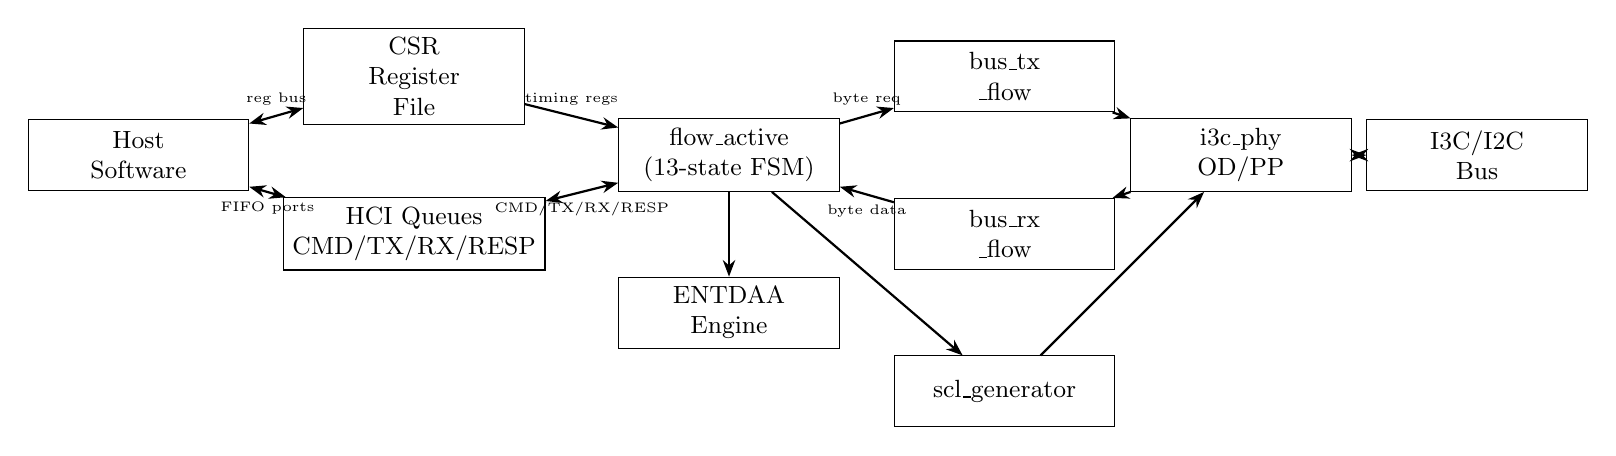
\begin{tikzpicture}[
  block/.style={rectangle, draw, minimum width=2.8cm, minimum height=0.9cm,
                align=center, font=\small},
  arrow/.style={-{Stealth[length=6pt]}, thick},
  darrow/.style={{Stealth[length=6pt]}-{Stealth[length=6pt]}, thick},
]
  % Host side
  \node[block] (host)     at (0, 0)    {Host\\Software};
  \node[block] (csr)      at (3.5, 1)  {CSR\\Register\\File};
  \node[block] (hci)      at (3.5, -1) {HCI Queues\\CMD/TX/RX/RESP};

  % Controller core
  \node[block] (fa)       at (7.5, 0)  {flow\_active\\(13-state FSM)};
  \node[block] (entdaa)   at (7.5, -2) {ENTDAA\\Engine};
  \node[block] (tx)       at (11, 1)   {bus\_tx\\\_flow};
  \node[block] (rx)       at (11, -1)  {bus\_rx\\\_flow};
  \node[block] (scl)      at (11, -3)  {scl\_generator};

  % PHY
  \node[block] (phy)      at (14, 0)   {i3c\_phy\\OD/PP};

  % Bus
  \node[block] (bus)      at (17, 0)   {I3C/I2C\\Bus};

  % Arrows
  \draw[darrow] (host) -- node[above,font=\tiny]{reg bus} (csr);
  \draw[darrow] (host) -- node[below,font=\tiny]{FIFO ports} (hci);
  \draw[arrow]  (csr)  -- node[above,font=\tiny]{timing regs} (fa);
  \draw[darrow] (hci)  -- node[below,font=\tiny]{CMD/TX/RX/RESP} (fa);
  \draw[arrow]  (fa)   -- node[above,font=\tiny]{byte req} (tx);
  \draw[arrow]  (rx)   -- node[below,font=\tiny]{byte data} (fa);
  \draw[arrow]  (fa)   -- (scl);
  \draw[arrow]  (fa)   -- (entdaa);
  \draw[arrow]  (tx)   -- (phy);
  \draw[arrow]  (phy)  -- (rx);
  \draw[arrow]  (scl)  -- (phy);
  \draw[darrow] (phy)  -- (bus);
\end{tikzpicture}
\caption{Top-level data flow diagram}
\label{fig:block_diagram}
\end{figure}

\section{Register Interface}

The host interface is a simple 32-bit synchronous register bus --- no AXI or AHB
protocol overhead.

\begin{table}[H]
\centering
\caption{Register bus interface signals}
\label{tab:reg_bus}
\begin{tabular}{llrl}
\toprule
\textbf{Signal} & \textbf{Dir.} & \textbf{Width} & \textbf{Description} \\
\midrule
\signal{reg\_addr\_i}  & Input  & 12 & Register address \\
\signal{reg\_wdata\_i} & Input  & 32 & Write data \\
\signal{reg\_wen\_i}   & Input  &  1 & Write enable \\
\signal{reg\_ren\_i}   & Input  &  1 & Read enable \\
\signal{reg\_rdata\_o} & Output & 32 & Read data \\
\signal{reg\_ready\_o} & Output &  1 & Transaction complete \\
\bottomrule
\end{tabular}
\end{table}

\section{Register Map}

\begin{table}[H]
\centering
\caption{CSR register map}
\label{tab:regmap}
\begin{tabularx}{\textwidth}{L{2.4cm} L{3.5cm} C{1.4cm} L{5.5cm}}
\toprule
\textbf{Address} & \textbf{Name} & \textbf{Access} & \textbf{Description} \\
\midrule
\texttt{0x000} & HC\_CONTROL    & RW & [0]=ENABLE; [1]=SW\_RESET (self-clearing) \\
\texttt{0x004} & HC\_STATUS     & RO & [0]=FSM\_IDLE; [1]=CMD\_FULL; [2]=RESP\_EMPTY \\
\texttt{0x010--0x030} & Timing (×9) & RW & 20-bit SCL timing registers \\
\texttt{0x100} & CMD\_QUEUE\_PORT & WO & 64-bit CMD via two 32-bit writes \\
\texttt{0x104} & TX\_DATA\_PORT & WO & Push to TX FIFO \\
\texttt{0x108} & RX\_DATA\_PORT & RO & Pop from RX FIFO \\
\texttt{0x10C} & RESP\_PORT     & RO & Pop from RESP FIFO \\
\texttt{0x110} & QUEUE\_STATUS  & RO & 8-bit FIFO flags \\
\texttt{0x200--0x23C} & DAT[0..15] & RW & 32-bit Device Address Table entries \\
\bottomrule
\end{tabularx}
\end{table}

The 64-bit command staging uses two consecutive 32-bit writes: the first write latches
DWORD0; the second write pushes \lstinline[style=plain]|{DWORD1, DWORD0}| as a 64-bit
command descriptor into the CMD FIFO.

\section{HCI Queue Architecture}

Four synchronous FIFOs form the data path between the host and the controller:

\begin{table}[H]
\centering
\caption{HCI FIFO configuration}
\label{tab:hci_fifos}
\begin{tabular}{lllrl}
\toprule
\textbf{Queue} & \textbf{Direction} & \textbf{Width} & \textbf{Depth} & \textbf{Purpose} \\
\midrule
CMD FIFO  & SW $\rightarrow$ HW & 64-bit & 64 & Command descriptors \\
TX FIFO   & SW $\rightarrow$ HW & 32-bit & 64 & Write data payload \\
RX FIFO   & HW $\rightarrow$ SW & 32-bit & 64 & Read data payload \\
RESP FIFO & HW $\rightarrow$ SW & 32-bit & 64 & Completion status \\
\bottomrule
\end{tabular}
\end{table}

\section{Command and Response Descriptors}

\subsection{Command Descriptor (64-bit)}

\begin{table}[H]
\centering
\caption{CMD FIFO descriptor field encoding}
\label{tab:cmd_desc}
\begin{tabular}{L{3cm} L{2.5cm} L{7cm}}
\toprule
\textbf{Field} & \textbf{Bits} & \textbf{Description} \\
\midrule
\texttt{cmd\_attr} & {[2:0]}  & Type: 000=Regular, 001=Immediate, 010=AddrAssign \\
\texttt{tid}       & {[6:3]}  & Transaction ID (echoed in response) \\
\texttt{dat\_index}& {[18:16]}& Index into Device Address Table (0--15) \\
\texttt{rnw}       & {[28]}   & 0=Write, 1=Read \\
\texttt{toc}       & {[30]}   & Terminate on completion (issue STOP) \\
\texttt{cp}        & {[31]}   & CCC present (prepend 0x7E broadcast header) \\
\texttt{data\_length}& {[47:32]}& Byte count for regular transfers \\
\texttt{imm\_data} & {[63:48]}& Inline data for immediate transfers (up to 4\,B) \\
\bottomrule
\end{tabular}
\end{table}

\subsection{Response Descriptor (32-bit)}

\begin{table}[H]
\centering
\caption{RESP FIFO descriptor field encoding}
\label{tab:resp_desc}
\begin{tabular}{L{3.5cm} L{2.5cm} L{6.5cm}}
\toprule
\textbf{Field} & \textbf{Bits} & \textbf{Description} \\
\midrule
\texttt{data\_length} & {[15:0]}  & Bytes transferred \\
\texttt{tid}          & {[27:24]} & Transaction ID (from command) \\
\texttt{err\_status}  & {[31:28]} & Error code \\
\bottomrule
\end{tabular}
\end{table}

Error codes: \texttt{0x0}=Success, \texttt{0x2}=Parity Error, \texttt{0x3}=Frame
Error, \texttt{0x4}=Address Header Error, \texttt{0x5}=NACK, \texttt{0x6}=Overflow.

\section{Signal Conventions}

\begin{itemize}
  \item Port suffixes: \signal{\_i} (input), \signal{\_o} (output)
  \item Reset: active-low asynchronous \signal{rst\_ni}
  \item FIFO handshake: \signal{*\_valid} / \signal{*\_ready}
  \item Bus inputs: \signal{scl\_i}, \signal{sda\_i} (2FF-synchronized)
  \item Bus outputs: \signal{scl\_o}, \signal{sda\_o} (active-low open-drain logic)
  \item \signal{sel\_od\_pp\_o}: 1\,=\,push-pull, 0\,=\,open-drain
\end{itemize}

% ==============================================================
\chapter{RTL Implementation}
% ==============================================================

\section{Overview}

The RTL is implemented in 18 SystemVerilog source files totaling approximately 4\,100
lines, organized across four implementation phases. Table~\ref{tab:rtl_files} lists
all files with their line counts.

\begin{table}[H]
\centering
\caption{RTL source file inventory}
\label{tab:rtl_files}
\begin{tabular}{L{6cm} rL{5cm}}
\toprule
\textbf{File} & \textbf{Lines} & \textbf{Phase} \\
\midrule
\file{i3c\_pkg.sv}              & 172 & Phase 0: Packages \\
\file{ctrl/controller\_pkg.sv}  &  20 & Phase 0: Packages \\
\file{phy/i3c\_phy.sv}          &  52 & Phase 1: Leaf \\
\file{ctrl/edge\_detector.sv}   &  39 & Phase 1: Leaf \\
\file{ctrl/stable\_high\_detector.sv} & 44 & Phase 1: Leaf \\
\file{ctrl/bus\_monitor.sv}     & 227 & Phase 1: Leaf \\
\file{ctrl/bus\_tx.sv}          & 185 & Phase 1: Leaf \\
\file{ctrl/bus\_tx\_flow.sv}    & 193 & Phase 1: Leaf \\
\file{ctrl/bus\_rx\_flow.sv}    & 166 & Phase 1: Leaf \\
\file{scl\_generator.sv}        & 257 & Phase 1: Leaf \\
\file{hci/sync\_fifo.sv}        &  84 & Phase 2: Infrastructure \\
\file{hci/hci\_queues.sv}       & 142 & Phase 2: Infrastructure \\
\file{csr/csr\_register.sv}     & 266 & Phase 2: Infrastructure \\
\file{ctrl/entdaa\_fsm.sv}      & 234 & Phase 3: Protocol \\
\file{ctrl/entdaa\_controller.sv} & 241 & Phase 3: Protocol \\
\file{ctrl/flow\_active.sv}     & 1\,166 & Phase 3: Protocol \\
\file{ctrl/controller\_active.sv} & 323 & Phase 4: Integration \\
\file{i3c\_controller\_top.sv}  & 261 & Phase 4: Integration \\
\midrule
\textbf{Total}                  & \textbf{4\,372} & \\
\bottomrule
\end{tabular}
\end{table}

\section{Shared Type Packages}

\subsection{i3c\_pkg.sv}

Defines top-level shared types including:
\begin{itemize}
  \item \texttt{bus\_state\_t}: composite struct carrying SCL/SDA value and stability
        flags from \module{bus\_monitor}.
  \item \texttt{i3c\_cmd\_attr\_e}: 3-bit enum for command type (Regular, Immediate,
        AddrAssign).
  \item \texttt{i3c\_resp\_err\_status\_e}: 4-bit error code enum.
  \item Command descriptor structs for each command type.
  \item \texttt{localparam logic [6:0] I3C\_RSVD\_ADDR = 7'h7E}.
\end{itemize}

\subsection{controller\_pkg.sv}

Defines controller-internal types, including the simplified 32-bit \texttt{dat\_entry\_t}:

\begin{lstlisting}[language=SystemVerilog, caption={Simplified 32-bit DAT entry type}]
typedef struct packed {
  logic        device;        // [31] 1 = I2C legacy device
  logic [8:0]  reserved;      // [30:22]
  logic [6:0]  dynamic_addr;  // [22:16] I3C dynamic address
  logic [9:0]  reserved2;     // [15:7]
  logic [6:0]  static_addr;   // [6:0]  I2C static address
} dat_entry_t;
\end{lstlisting}

This reduces DAT memory from 128\,B (reference 64-bit entries) to 64\,B for 16
devices while retaining all required fields.

\section{Physical Layer}

\file{i3c\_phy.sv} (52 lines) handles the physical bus interface with two
responsibilities.

\textbf{Input synchronization:} A two-flip-flop synchronizer chains
$d \rightarrow \text{ff1} \rightarrow \text{ff2}$ on both SCL and SDA inputs to
mitigate metastability at the asynchronous bus/clock-domain boundary.

\textbf{Output driver:} Implements open-drain and push-pull modes under
\signal{sel\_od\_pp\_i} control:
\begin{itemize}
  \item \textbf{Open-drain} (\signal{sel\_od\_pp\_i\,=\,0}): SDA driven LOW when
        \signal{sda\_o\,=\,0}, else tri-stated (high-impedance).
  \item \textbf{Push-pull} (\signal{sel\_od\_pp\_i\,=\,1}): active drive of both
        HIGH and LOW, enabling 12.5\,MHz operation.
\end{itemize}

\section{SCL Generator}

\file{scl\_generator.sv} (257 lines) is a new module implementing a 13-state FSM to
generate START, clock, repeated START, and STOP conditions:

\begin{figure}[H]
\centering
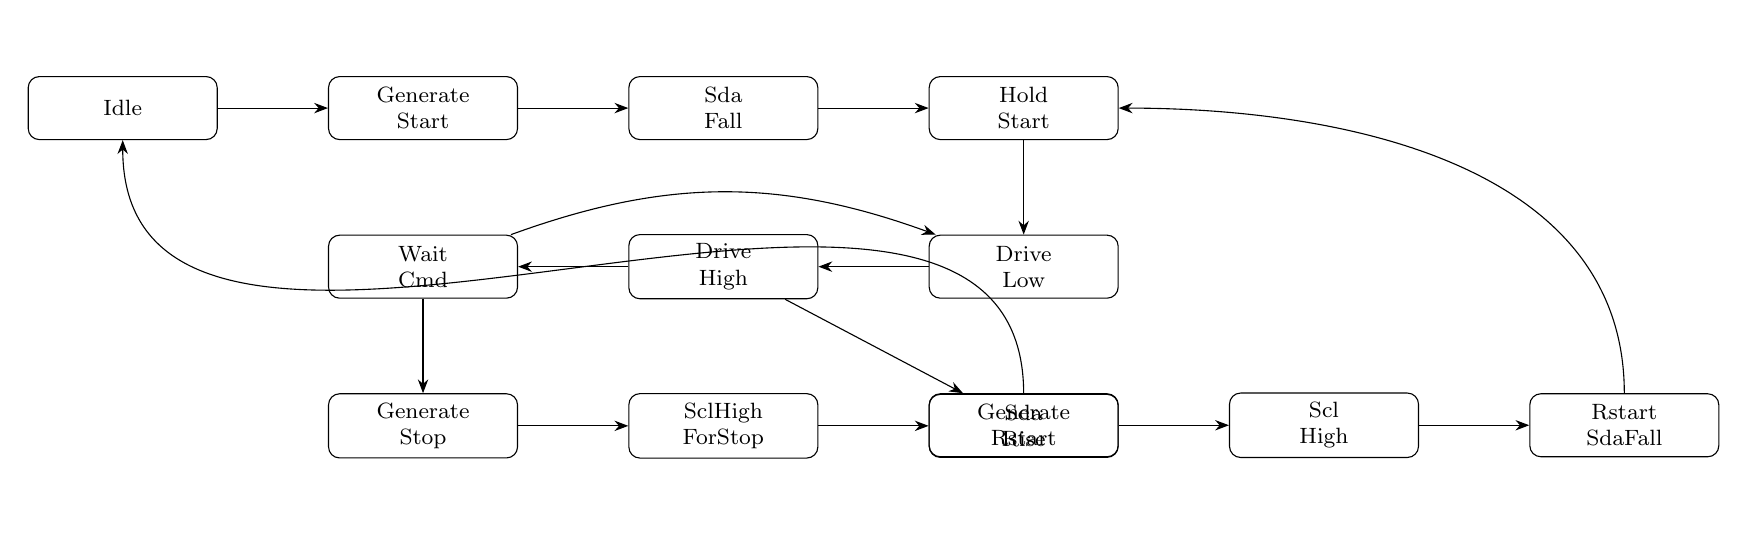
\begin{tikzpicture}[
  s/.style={rectangle, draw, rounded corners, minimum width=2.4cm,
            minimum height=0.8cm, align=center, font=\footnotesize},
  a/.style={-{Stealth[length=5pt]}, font=\tiny},
  node distance=1.2cm and 1.4cm,
]
  \node[s] (idle)   {Idle};
  \node[s, right=of idle]  (gstart)  {Generate\\Start};
  \node[s, right=of gstart] (sdafall) {Sda\\Fall};
  \node[s, right=of sdafall] (hold)   {Hold\\Start};
  \node[s, below=of hold]  (dlow)    {Drive\\Low};
  \node[s, left=of dlow]   (dhigh)   {Drive\\High};
  \node[s, left=of dhigh]  (wcmd)    {Wait\\Cmd};

  \node[s, below=of dlow]  (grst)    {Generate\\Rstart};
  \node[s, right=of grst]  (sclhigh) {Scl\\High};
  \node[s, right=of sclhigh] (rsda)  {Rstart\\SdaFall};

  \node[s, below=of wcmd]  (gstop)   {Generate\\Stop};
  \node[s, right=of gstop] (sclstp)  {SclHigh\\ForStop};
  \node[s, right=of sclstp] (srise)  {Sda\\Rise};

  \draw[a] (idle) -- (gstart);
  \draw[a] (gstart) -- (sdafall);
  \draw[a] (sdafall) -- (hold);
  \draw[a] (hold) -- (dlow);
  \draw[a] (dlow) -- (dhigh);
  \draw[a] (dhigh) -- (wcmd);
  \draw[a] (wcmd) to[bend left=20] (dlow);

  \draw[a] (dhigh) -- (grst);
  \draw[a] (grst) -- (sclhigh);
  \draw[a] (sclhigh) -- (rsda);
  \draw[a] (rsda) to[out=90, in=0] (hold);

  \draw[a] (wcmd) -- (gstop);
  \draw[a] (gstop) -- (sclstp);
  \draw[a] (sclstp) -- (srise);
  \draw[a] (srise) to[out=90, in=-90] (idle);
\end{tikzpicture}
\caption{SCL generator 13-state FSM}
\label{fig:scl_fsm}
\end{figure}

A single countdown counter \signal{tcount} loads a state-dependent initial value from
the timing registers and decrements each clock cycle. State transitions occur only when
\signal{tcount} reaches zero, precisely meeting I3C/I2C setup and hold time
requirements. The selector \signal{sel\_i3c\_i2c\_i} chooses between the I3C (12.5\,MHz)
and I2C (400\,kHz) timing register banks.

\section{Bus TX and RX Paths}

\subsection{TX Path}

\textbf{\file{bus\_tx.sv}} (185 lines) is the bit-level TX engine. It drives SDA
synchronized to SCL edges in three steps: (1) wait for \signal{scl\_stable\_low\_i};
(2) set up SDA with the bit value (setup time before SCL rise); (3) hold SDA through
SCL HIGH; (4) pulse \signal{done\_o} on SCL fall.

\textbf{\file{bus\_tx\_flow.sv}} (193 lines) is the byte serializer. A 4-state FSM
unpacks a byte, drives bits MSB-first, and generates the T-bit (parity or ACK). The
module accepts either full-byte requests (\signal{req\_byte\_i}) or single-bit
requests (\signal{req\_bit\_i}).

\subsection{RX Path}

\textbf{\file{bus\_rx\_flow.sv}} (166 lines) deserializes bits from SDA into bytes.
A 4-state FSM samples SDA on each SCL positive edge and assembles 8-bit bytes
MSB-first. The received byte and T-bit are available on \signal{rx\_data\_o} and
\signal{rx\_t\_bit\_o}.

\section{HCI Queues}

\textbf{\file{sync\_fifo.sv}} (84 lines) is a parameterized synchronous FIFO using
the extra-MSB pointer technique for empty/full detection:

\begin{lstlisting}[language=SystemVerilog, caption={FIFO full/empty detection}]
assign empty_o = (wptr_q == rptr_q);
assign full_o  = (rptr_q == {~wptr_q[PtrW], wptr_q[PtrW-1:0]});
\end{lstlisting}

This technique requires \texttt{Depth} to be a power of two, enforced by a compile-time
\lstinline{$fatal} assertion. \textbf{\file{hci\_queues.sv}} (142 lines) instantiates
four \module{sync\_fifo} instances with widths and depths from Table~\ref{tab:hci_fifos}.

\section{CSR Register File}

\file{csr\_register.sv} (266 lines) is a hand-written register file replacing the
14\,342-line auto-generated reference. Key implementation points:

\begin{itemize}
  \item \textbf{CMD staging}: \signal{cmd\_staging\_valid\_q} tracks whether DWORD0
        has been latched. On second write, pushes \lstinline|{DWORD1, DWORD0}| as a
        64-bit command descriptor.
  \item \textbf{RX/RESP reads}: assert \signal{rready} to pop the FIFO on the read
        access cycle, providing zero-latency FIFO access.
  \item \textbf{SW\_RESET}: self-clearing; also clears \signal{cmd\_staging\_valid\_q}
        and \signal{cmd\_dword0\_q} to prevent stale command corruption.
  \item \textbf{Timing defaults}: preloaded for 333\,MHz/I3C 12.5\,MHz operation.
\end{itemize}

\section{ENTDAA Engine}

\subsection{entdaa\_fsm.sv}

\file{entdaa\_fsm.sv} (234 lines) is a complete rewrite of the reference
\file{ccc\_entdaa.sv}. The reference is a \emph{target-side} implementation (transmits
64-bit identity, receives assigned address). The thesis rewrites this as a
\emph{master-side} FSM (receives the arbitration bits, transmits the assigned address):

\begin{table}[H]
\centering
\caption{Master-side ENTDAA FSM states}
\label{tab:entdaa_states}
\begin{tabularx}{\textwidth}{L{3cm} L{9.5cm}}
\toprule
\textbf{State} & \textbf{Action} \\
\midrule
\state{Idle}        & Wait for \signal{start\_daa\_i} \\
\state{WaitStart}   & Wait for \signal{rstart\_det\_i} (Sr from \module{flow\_active}) \\
\state{ReceiveIDBit}& Assert \signal{rx\_req\_bit}; receive 64 bits (PID + BCR + DCR) \\
\state{SendAddr}    & Assert \signal{tx\_req\_byte}; send \texttt{\{7-bit addr, parity\}} \\
\state{WaitAck}     & Assert \signal{rx\_req\_bit}; read ACK from winning target \\
\state{Done}        & Pulse \signal{done\_daa\_o}; present PID/BCR/DCR outputs \\
\state{Error}       & On NACK or timeout \\
\bottomrule
\end{tabularx}
\end{table}

\subsection{entdaa\_controller.sv}

\file{entdaa\_controller.sv} (241 lines) manages the multi-device ENTDAA loop.
It instantiates \module{entdaa\_fsm} and iterates until all devices in
\signal{dev\_count\_i} have been addressed. For each round, it looks up the
pre-assigned address from the DAT and passes it to the FSM.

\section{Command FSM (flow\_active.sv)}

\file{flow\_active.sv} (1\,166 lines) is the most critical module, implementing
the 13-state command FSM that orchestrates all master transactions. The reference
contained 8 unimplemented TODO states; the thesis implements all 13:

\begin{lstlisting}[language=SystemVerilog, caption={flow\_active FSM state enumeration}]
typedef enum logic [3:0] {
  Idle,               // Waiting for command
  WaitForCmd,         // Pop and decode CMD FIFO
  FetchDAT,           // Look up DAT entry
  I3CWriteImmediate,  // I3C immediate write (inline data)
  I2CWriteImmediate,  // I2C immediate write
  FetchTxData,        // Pop TX FIFO (one DWORD)
  FetchRxData,        // Push accumulated bytes to RX FIFO
  InitI2CWrite,       // I2C: START + addr + W + ACK
  InitI2CRead,        // I2C: START + addr + R + ACK
  StallWrite,         // Clock-stall: TX FIFO empty
  StallRead,          // Clock-stall: RX FIFO full
  IssueCmd,           // Main data transfer workhorse
  WriteResp           // Push response to RESP FIFO
} flow_fsm_state_e;
\end{lstlisting}

Table~\ref{tab:flow_states} describes the responsibility of each state. All 8 states
that were TODO stubs in the reference are implemented here for the first time.

\begin{table}[H]
\centering
\caption{flow\_active FSM state responsibilities}
\label{tab:flow_states}
\begin{tabularx}{\textwidth}{L{4.2cm} C{2.4cm} L{6cm}}
\toprule
\textbf{State} & \textbf{Ref. Status} & \textbf{Implementation} \\
\midrule
\state{Idle}             & Done    & Assert \signal{fsm\_idle\_o}; wait CMD \\
\state{WaitForCmd}       & Done    & Pop CMD FIFO; decode descriptor \\
\state{FetchDAT}         & Done    & Index DAT; wait one cycle for registered read \\
\state{I2CWriteImmediate}& Partial & START(OD) + addr + inline bytes \\
\state{I3CWriteImmediate}& TODO    & START + bcast header + dyn addr + inline bytes with T-bit \\
\state{FetchTxData}      & TODO    & Pop TX FIFO; go to IssueCmd or StallWrite \\
\state{FetchRxData}      & TODO    & Write RX DWORD to RX FIFO; continue or stall \\
\state{InitI2CWrite}     & TODO    & START(OD) + \{static\_addr, W\} + read ACK \\
\state{InitI2CRead}      & TODO    & START(OD) + \{static\_addr, R\} + read ACK \\
\state{StallWrite}       & TODO    & Deassert \signal{gen\_clock}; poll TX FIFO non-empty \\
\state{StallRead}        & TODO    & Deassert \signal{gen\_clock}; poll RX FIFO space \\
\state{IssueCmd}         & TODO    & Serialize writes; receive reads; ENTDAA delegation \\
\state{WriteResp}        & Done    & Push error code + byte count to RESP FIFO \\
\bottomrule
\end{tabularx}
\end{table}

\textbf{OD/PP switching} is controlled by \signal{sel\_od\_pp\_q}:
\begin{itemize}
  \item Open-drain: address phase and ACK sampling
  \item Push-pull: I3C data byte transmission/reception
  \item Always open-drain: I2C transactions
  \item Transitions are gated behind \signal{bus\_tx\_idle} --- never mid-byte
\end{itemize}

\textbf{Issue phases} within \state{IssueCmd} are tracked by \signal{issue\_phase\_q},
an 8-bit counter that sequences through START $\rightarrow$ address $\rightarrow$ data
bytes $\rightarrow$ STOP, keeping TX and RX operations in distinct cycles.

\section{Controller Wrapper (controller\_active.sv)}

\file{controller\_active.sv} (323 lines) instantiates and connects all protocol
sub-modules. Key combinational logic blocks:

\textbf{SDA multiplexer:}
\begin{lstlisting}[language=SystemVerilog, caption={SDA output multiplexer}]
assign sda_o = scl_gen_busy ? scl_gen_sda_o
             : tx_active    ? bus_tx_sda_o
                            : 1'b1;  // release bus
\end{lstlisting}

The SCL generator takes SDA ownership during START/STOP generation; \module{bus\_tx}
drives SDA during data phases; default is HIGH (bus released).

\textbf{Arbitration detection:}
\begin{lstlisting}[language=SystemVerilog, caption={Arbitration lost detection}]
assign arbitration_lost = tx_sda_driven & ~bus_state.sda.value;
\end{lstlisting}

Detects when the master drives HIGH but reads LOW on SDA.

% ==============================================================
\chapter{Functional Verification}
% ==============================================================

\section{Verification Strategy}

The verification environment targets functional coverage of all implemented features
using the \textbf{UVM (Universal Verification Methodology)} framework with
\textbf{Xcelium} (Cadence, UVM 1.2 CDNS-1.2 bundled) as the simulator.

Verification is structured in two phases:
\begin{itemize}
  \item \textbf{Phase 1 (implemented):} Register agent infrastructure and basic
        I3C write/read transfers.
  \item \textbf{Phase 2 (planned):} ENTDAA sequence, CCC commands, I2C legacy,
        error injection, multi-device, functional coverage groups.
\end{itemize}

\section{Environment Architecture}

Figure~\ref{fig:uvm_env} shows the UVM environment hierarchy.

\begin{figure}[H]
\centering
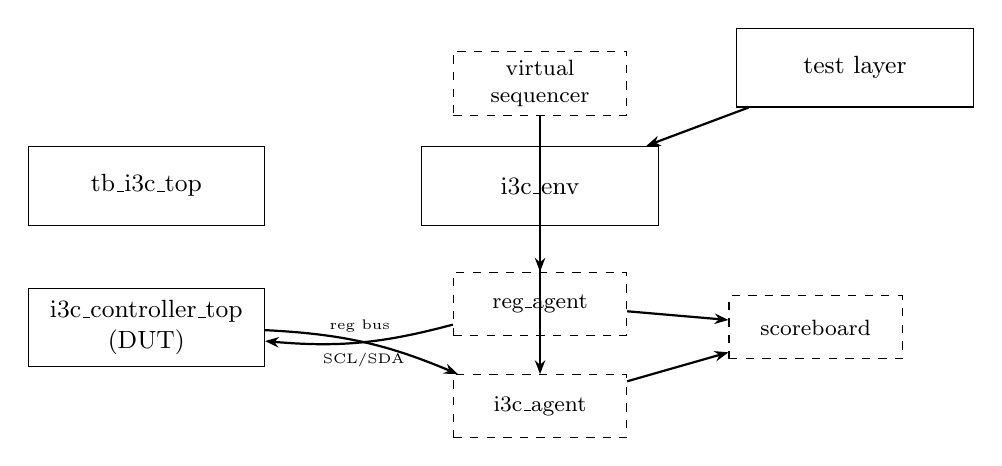
\begin{tikzpicture}[
  box/.style={rectangle, draw, minimum width=3cm, minimum height=1cm,
              align=center, font=\small},
  subbox/.style={rectangle, draw, dashed, minimum width=2.2cm, minimum height=0.8cm,
                 align=center, font=\footnotesize},
  arrow/.style={-{Stealth[length=5pt]}, thick},
  node distance=1.2cm and 1.4cm,
]
  \node[box] (tb)     at (0, 0)    {tb\_i3c\_top};
  \node[box] (dut)    at (0, -1.8) {i3c\_controller\_top\\(DUT)};
  \node[box] (env)    at (5, 0)    {i3c\_env};
  \node[subbox] (ra)  at (5, -1.5) {reg\_agent};
  \node[subbox] (ia)  at (5, -2.8) {i3c\_agent};
  \node[subbox] (vs)  at (5, 1.3)  {virtual\\sequencer};
  \node[subbox] (scb) at (8.5, -1.8) {scoreboard};
  \node[box] (test)   at (9, 1.5)  {test layer};

  \draw[arrow] (test) -- (env);
  \draw[arrow] (vs) -- (ra);
  \draw[arrow] (vs) -- (ia);
  \draw[arrow] (ra) to[bend left=10] node[above,font=\tiny]{reg bus} (dut);
  \draw[arrow] (dut) to[bend left=10] node[below,font=\tiny]{SCL/SDA} (ia);
  \draw[arrow] (ra) -- (scb);
  \draw[arrow] (ia) -- (scb);
\end{tikzpicture}
\caption{UVM environment architecture}
\label{fig:uvm_env}
\end{figure}

\section{Register Agent}

The register agent provides test infrastructure for the simple register bus interface.
Table~\ref{tab:reg_agent} lists the Phase 1 components that have been implemented.

\begin{table}[H]
\centering
\caption{Register agent components (Phase 1, implemented)}
\label{tab:reg_agent}
\begin{tabularx}{\textwidth}{L{4.5cm} L{8.5cm}}
\toprule
\textbf{File} & \textbf{Description} \\
\midrule
\file{reg\_if.sv}           & SystemVerilog interface: addr/wdata/wen/ren/rdata/ready \\
\file{reg\_seq\_item.sv}    & UVM sequence item: one register transaction \\
\file{reg\_driver.sv}       & Drives interface; asserts valid for one cycle per transaction \\
\file{reg\_monitor.sv}      & Samples completed transactions; sends to analysis port \\
\file{reg\_sequencer.sv}    & Standard \texttt{uvm\_sequencer} \\
\file{reg\_agent.sv}        & Top-level agent: instantiates driver, monitor, sequencer \\
\file{reg\_agent\_cfg.sv}   & Agent configuration object \\
\file{reg\_agent\_pkg.sv}   & Collects all agent components into one package \\
\file{i3c\_csr\_addr\_pkg.sv} & Named address constants (\texttt{ADDR\_HC\_CONTROL}, etc.) \\
\bottomrule
\end{tabularx}
\end{table}

\section{I3C Bus Agent}

The I3C agent operates in \textbf{device (target) mode} --- it responds to
master-driven bus activity rather than initiating transfers:
\begin{itemize}
  \item \textbf{Driver:} samples SCL edges; drives SDA during ACK phases and
        ENTDAA arbitration.
  \item \textbf{Monitor:} captures complete I3C frames (START to STOP); constructs
        \texttt{i3c\_item} objects for the scoreboard.
  \item \textbf{Device response sequence:} automatic ACK/NACK, ENTDAA PID
        broadcasting, T-bit generation.
\end{itemize}

\section{Scoreboard}

The scoreboard performs end-to-end checking:
\begin{itemize}
  \item \textbf{Write check:} compares data observed on the I3C bus against the TX
        FIFO contents written by the test sequence.
  \item \textbf{Read check:} compares data written to the RX FIFO against data
        driven by the I3C device driver.
  \item \textbf{Response check:} verifies RESP FIFO \texttt{err\_status\,==\,Success}
        and \texttt{data\_length} matches the command descriptor.
\end{itemize}

\section{Phase 1 Test Plan}

\begin{table}[H]
\centering
\caption{Phase 1 test scenarios}
\label{tab:phase1_tests}
\begin{tabularx}{\textwidth}{L{2.5cm} L{3.5cm} L{3.5cm} L{3cm}}
\toprule
\textbf{Test} & \textbf{Sequence} & \textbf{Scenario} & \textbf{Pass Criteria} \\
\midrule
\texttt{i3c\_smoke} & \texttt{i3c\_smoke\_vseq} & 1-byte immediate write & Bus active; RESP=Success \\
\texttt{i3c\_write} & \texttt{i3c\_write\_vseq} & N-byte regular write via TX FIFO & Bus data = TX data; RESP=Success \\
\texttt{i3c\_read}  & \texttt{i3c\_read\_vseq}  & N-byte regular read to RX FIFO  & RX data = device data; RESP=Success \\
\bottomrule
\end{tabularx}
\end{table}

The standard test sequence flow is:

\begin{enumerate}
  \item Configure timing registers (use CSR defaults for 333\,MHz / 12.5\,MHz)
  \item Write DAT entry with device dynamic address
  \item Enable controller (\texttt{HC\_CONTROL[0]\,=\,1})
  \item Write CMD descriptor (two 32-bit writes to \texttt{CMD\_QUEUE\_PORT})
  \item Write TX data to \texttt{TX\_DATA\_PORT} (for write commands)
  \item Fork \texttt{i3c\_device\_response\_seq} on the I3C bus agent
  \item DUT drives: START $\rightarrow$ address $\rightarrow$ data $\rightarrow$ STOP
  \item Poll \texttt{HC\_STATUS[2]} (RESP\_EMPTY); read \texttt{RESP\_PORT}
  \item Scoreboard checks all observations
\end{enumerate}

\section{Build Infrastructure}

\begin{lstlisting}[style=plain, caption={Xcelium build and run commands}]
# Compile + elaborate
xrun -compile -elaborate \
     -f verification/uvm_i3c/filelist.f \
     -uvmhome CDNS-1.2

# Run smoke test
xrun -R +UVM_TESTNAME=i3c_base_test \
        +UVM_TEST_SEQ=i3c_smoke_vseq

# Run write test with verbosity
xrun -R +UVM_TESTNAME=i3c_base_test \
        +UVM_TEST_SEQ=i3c_write_vseq \
        +UVM_VERBOSITY=UVM_HIGH
\end{lstlisting}

\section{Phase 2 Roadmap}

\begin{table}[H]
\centering
\caption{Phase 2 verification roadmap}
\label{tab:phase2}
\begin{tabularx}{\textwidth}{C{0.5cm} L{3cm} L{8.5cm}}
\toprule
\textbf{\#} & \textbf{Feature} & \textbf{Description} \\
\midrule
1 & ENTDAA test    & Full DAA: bcast header $\rightarrow$ CCC $\rightarrow$ Sr $\rightarrow$ arbitration $\rightarrow$ addr assign \\
2 & Error injection & NACK from target; FIFO overflow; abort conditions \\
3 & CCC tests      & ENEC/DISEC broadcast and direct \\
4 & I2C legacy     & I2C device write/read at 400\,kHz \\
5 & Multi-device   & Multiple I3C targets; test DAT lookup \\
6 & Func. coverage & Covergroups: FSM transitions, CCC types, OD/PP, FIFO boundaries \\
\bottomrule
\end{tabularx}
\end{table}

% ==============================================================
\chapter{Bug Analysis and Fixes}
% ==============================================================

\section{Overview}

A systematic code review of all 18 RTL source files was conducted on April 27, 2026,
identifying 22 issues classified into four severity levels.

\begin{table}[H]
\centering
\caption{Bug severity summary}
\label{tab:bug_summary}
\begin{tabular}{lrl}
\toprule
\textbf{Severity} & \textbf{Count} & \textbf{Criteria} \\
\midrule
CRITICAL & 3 & Blocks synthesis or causes total functional failure \\
HIGH     & 8 & Incorrect protocol or logic behavior \\
MEDIUM   & 7 & Timing inconsistencies or incomplete features \\
LOW      & 4 & Style / maintainability \\
\midrule
\textbf{Total} & \textbf{22} & \\
\bottomrule
\end{tabular}
\end{table}

\section{Critical Issues}

\subsection*{BUG-001 --- Stray character in CSR parameter list}

\textbf{File:} \file{csr\_register.sv}, line 15.

A stray \texttt{/} character after the comma in the parameter list causes a parse
error and prevents all compilation:

\begin{lstlisting}[language=SystemVerilog]
// Buggy:
parameter int unsigned CmdDataWidth = 64,/

// Fixed:
parameter int unsigned CmdDataWidth = 64,
\end{lstlisting}

\subsection*{BUG-002 --- Missing SCL clock for immediate transfers}

\textbf{File:} \file{flow\_active.sv}, states \state{I2CWriteImmediate} and
\state{I3CWriteImmediate}. \textbf{Impact:} all immediate transfers hang after START.

\signal{gen\_clock\_q} is never asserted in the immediate states. After the START
condition, \module{scl\_generator} transitions to \state{WaitCmd} with
\signal{gen\_clock\,=\,0}, and SCL never toggles. The TX engine enters
\state{TransmitData} and waits indefinitely for SCL edges that never arrive.

\textbf{Fix:} Assert \signal{gen\_clock\_q\,=\,1'b1} at state entry:

\begin{lstlisting}[language=SystemVerilog]
I2CWriteImmediate: begin
  gen_clock_q  = 1'b1;  // <-- add this
  sel_i3c_i2c_q = 1'b0;
  sel_od_pp_q   = 1'b0;
  // ...
end
\end{lstlisting}

\subsection*{BUG-003 --- RX partial DWORD data loss on read transfers}

\textbf{File:} \file{flow\_active.sv}, states \state{IssueCmd} and
\state{FetchRxData}. \textbf{Impact:} silent data loss on any read whose length
is not a multiple of 4 bytes.

Received bytes are accumulated into \signal{rx\_dword\_q} four at a time and flushed
only on DWORD alignment. When a read completes (\signal{remaining\_len\_q\,==\,0}),
the FSM transitions to \state{WriteResp} without flushing any partial DWORD.

\textbf{Fix:} Flush before entering \state{WriteResp}:

\begin{lstlisting}[language=SystemVerilog]
if (remaining_len_q == '0) begin
  if (rx_byte_idx_q != 2'h0) begin  // partial DWORD pending
    rx_queue_wvalid_q = 1'b1;
    rx_queue_wdata_q  = rx_dword_q;
  end
  state_d = WriteResp;
end
\end{lstlisting}

\section{High-Severity Issues}

\subsection*{BUG-004/005/006 --- Same-cycle TX/RX dependency (three instances)}

\textbf{Files:} \file{flow\_active.sv}, I2C write (line 997--1011), I2C read
(line 1056--1074), I3C read (line 1089--1114).

In all three paths, \signal{bus\_rx\_req\_bit\_q} is asserted inside a
\signal{bus\_tx\_done\_i} condition block, then \signal{bus\_rx\_done\_i} is
checked within the same combinational block. Both signals are single-cycle pulses
generated by different modules; they cannot both be asserted in the same cycle.

\textbf{Impact:} ACK/NACK is never sampled for I2C writes, I2C reads, or I3C read
T-bit acknowledgement.

\textbf{Fix:} Use \signal{issue\_phase\_q} to separate TX and RX into distinct cycles:

\begin{lstlisting}[language=SystemVerilog]
// Phase 0: send byte
if (issue_phase_q[0] == 1'b0) begin
  bus_tx_req_byte_q  = 1'b1;
  bus_tx_req_value_q = current_tx_byte;
  if (bus_tx_done_i) issue_phase_d = issue_phase_q + 1;
// Phase 1: receive ACK
end else begin
  bus_rx_req_bit_q = 1'b1;
  if (bus_rx_done_i) begin
    nack_detected_d = bus_rx_data_i[0];
    issue_phase_d   = 8'h0;
  end
end
\end{lstlisting}

\subsection*{BUG-007 --- Missing START for I3C regular transfers}

\textbf{File:} \file{flow\_active.sv}, \state{IssueCmd} state. \textbf{Impact:}
all I3C regular write/read transfers produce illegal bus activity.

For \texttt{RegularTransfer} commands to I3C devices, \state{IssueCmd} immediately
serializes data bytes without first generating START or transmitting the address byte.

\textbf{Fix:} Add initial \signal{issue\_phase} steps in \state{IssueCmd} for I3C
regular transfers to generate START and send the address byte before data.

\subsection*{BUG-008 --- SW reset doesn't clear CMD staging}

\textbf{File:} \file{csr\_register.sv}, lines 162--179.

Software reset clears \signal{cmd\_wvalid\_q} but not \signal{cmd\_staging\_valid\_q}
or \signal{cmd\_dword0\_q}. A stale DWORD0 after reset will be paired with the next
write, producing a garbage 64-bit command.

\textbf{Fix:}
\begin{lstlisting}[language=SystemVerilog]
end else if (sw_reset_q || (cmd_wvalid_q && cmd_wready_i)) begin
  cmd_wvalid_q        <= '0;
  cmd_staging_valid_q <= '0;  // add
  cmd_dword0_q        <= '0;  // add
end
\end{lstlisting}

\subsection*{BUG-009 --- gen\_idle\_o never asserted}

\signal{gen\_idle\_q} defaults to \signal{1'b0} and is never set to \signal{1'b1}
in any state, eliminating the only bus-abort mechanism. Without this signal, a
stuck SCL generator (e.g., from target clock-stretching) cannot be recovered.

\subsection*{BUG-010 --- bus\_rx\_flow shift register data race}

\textbf{File:} \file{bus\_rx\_flow.sv}, lines 54 and 78.

Both the shift register and the output mux use raw \signal{sda\_i}. Since
\signal{rx\_done} fires one cycle after the SCL positive edge, \signal{sda\_i}
may have been updated to the next bit by the target.

\textbf{Fix:} Use the registered sample \signal{rx\_bit} in both locations.

\subsection*{BUG-011 --- FIFO non-power-of-2 depth}

The extra-MSB pointer technique silently malfunctions for non-power-of-2 depths.
The current default (64) is safe, but the constraint is implicit.

\textbf{Fix:} Add a compile-time assertion:
\begin{lstlisting}[language=SystemVerilog]
initial
  assert (Depth == (1 << PtrW))
    else $fatal(1, "sync_fifo: Depth must be a power of 2");
\end{lstlisting}

\section{Medium-Severity Issues}

\begin{description}
  \item[BUG-012/013] Off-by-one timing inconsistency between \module{edge\_detector}
    (\texttt{count >= delay}) and \module{stable\_high\_detector}
    (\texttt{count > delay}), producing a one-cycle asymmetry for equal
    \signal{delay\_count} values.

  \item[BUG-014] Missing \signal{gen\_rstart\_i} handling in \state{WaitCmd} of
    \module{scl\_generator}. A repeated START requested while SCL is held LOW will
    be silently dropped.

  \item[BUG-015] \signal{ccc\_code\_o} always outputs \texttt{0x00} because
    \signal{ccc\_code\_q} is never assigned from the descriptor's \texttt{cmd} field.

  \item[BUG-016] T-bit parity check for I3C reads uses a static comparison
    (\texttt{bus\_rx\_data\_i[0] != 1'b1}) instead of the correct XOR-based odd
    parity over the received byte.

  \item[BUG-017] Bitwise \texttt{\&} used instead of logical \texttt{\&\&} in
    \module{bus\_tx.sv} line 176.

  \item[BUG-018] \signal{rx\_req\_bit} registration asymmetry in
    \module{bus\_rx\_flow}: Idle$\rightarrow$ReadBit uses the registered signal,
    but the abort logic uses the unregistered input.
\end{description}

\section{Low-Severity Issues}

\begin{description}
  \item[BUG-019] Counter underflow in \module{entdaa\_fsm}: \signal{bit\_cnt\_d}
    decrements below zero on the final bit. Benign in current design but fragile
    if reused.
  \item[BUG-020] Signals using \signal{\_q} suffix in \module{flow\_active} are
    assigned combinationally, violating the project's \signal{\_q}=registered naming
    convention.
  \item[BUG-021] Verilog-2001 \texttt{wire} keyword used in
    \module{controller\_active} instead of SystemVerilog \texttt{logic}.
  \item[BUG-022] ENTDAA CCC code hardcoded as \texttt{8'h07} in
    \module{flow\_active} instead of a named constant from \file{i3c\_pkg.sv}.
\end{description}

\section{Remediation Priority}

\begin{enumerate}
  \item \textbf{BUG-001}: Fix first --- syntax error blocks all subsequent work.
  \item \textbf{BUG-002, BUG-003}: Fix before first simulation --- makes immediate
        transfers and non-aligned reads completely non-functional.
  \item \textbf{BUG-004 through BUG-008}: Fix for correct protocol behavior in all
        transfer modes.
  \item \textbf{BUG-009 through BUG-011}: Fix for robustness.
  \item \textbf{BUG-012 through BUG-022}: Can be deferred but should be tracked.
\end{enumerate}

% ==============================================================
\chapter{Results and Discussion}
% ==============================================================

\section{Design Metrics}

Table~\ref{tab:metrics} summarizes the key metrics of the completed design.

\begin{table}[H]
\centering
\caption{Design metrics summary}
\label{tab:metrics}
\begin{tabular}{lr}
\toprule
\textbf{Metric} & \textbf{Value} \\
\midrule
RTL source files                 & 18 \\
Total RTL lines                  & $\sim$4\,100 \\
Phase 1 verification files       & 9 \\
Phase 1 verification lines       & $\sim$353 \\
Reference design LoC             & $\sim$25\,000 \\
Code reduction vs.\ reference    & $\sim$84\% \\
FSM states implemented           & 13 / 13 \\
FSM states in reference          & 5 / 13 \\
Bugs identified                  & 22 \\
\quad Critical                   & 3 \\
\quad High                       & 8 \\
\quad Medium                     & 7 \\
\quad Low                        & 4 \\
\bottomrule
\end{tabular}
\end{table}

\section{Design Contributions}

This thesis makes six original contributions relative to the CHIPS Alliance reference.

\subsection{Complete Command FSM}

The thesis is the first complete implementation of the 13-state \module{flow\_active}
FSM. The reference left 8 of 13 states as TODO stubs, making it non-functional for
regular I3C and I2C transfers, FIFO stalling, and RX data accumulation. The thesis
implements all missing states, adding approximately 600 lines of original protocol logic.

\subsection{Register File Redesign}

The 14\,342-line auto-generated CSR is replaced by a 266-line hand-written register
file --- a 98\% reduction. The hand-written approach is human-readable, auditable,
directly synthesizable, and covers all registers needed for the thesis scope without
Caliptra-specific fields.

\subsection{OD/PP Driver Switching}

The reference hardcodes open-drain mode, making 12.5\,MHz SDR physically impossible.
The thesis implements proper OD/PP switching in \module{flow\_active} (via
\signal{sel\_od\_pp\_q}) and routes it through \module{controller\_active} to the PHY
--- a prerequisite for any I3C SDR data transfer.

\subsection{Master-Side ENTDAA FSM}

The reference \file{entdaa\_fsm.sv} is target-side: it transmits the device's 64-bit
identity and receives an assigned address. The thesis completely rewrites this as a
master-side FSM: receiving arbitration identity bits and transmitting the assigned
address. All TX/RX roles, counter directions, and state transitions are inverted
relative to the reference.

\subsection{Infrastructure Simplification}

AXI4 + AHB adapters (700+ lines) are replaced by a simple register bus (50 lines).
The 2\,500+ line threshold-based HCI queue system is replaced by four 84-line
synchronous FIFOs. Top-level \texttt{\#ifdef} conditional compilation with 50+
parameters is replaced by a clean parameterized hierarchy.

\subsection{Systematic Bug Documentation}

A formal bug analysis identifies 22 issues with root-cause analysis and recommended
fixes, providing a clear remediation roadmap for the verification phase.

\section{Architectural Trade-offs}

\begin{table}[H]
\centering
\caption{Key architectural decisions and trade-offs}
\label{tab:tradeoffs}
\begin{tabularx}{\textwidth}{L{4cm} L{4cm} L{5cm}}
\toprule
\textbf{Decision} & \textbf{Choice} & \textbf{Trade-off} \\
\midrule
Clock domain   & Single 333\,MHz clock       & No CDC complexity; requires fast process \\
Bus interface  & Simple 32-bit register bus  & Easy to verify; not AXI-compatible for SoC \\
DAT depth      & 16 entries (vs.\ 128)       & Sufficient for thesis; limits bus to 16 devices \\
I2C timing     & Hardcoded 400\,kHz          & Reduces CSR; no runtime I2C configurability \\
FIFO type      & Synchronous                 & Eliminates CDC; single-clock design \\
\bottomrule
\end{tabularx}
\end{table}

\section{Limitations}

\textbf{Simulation not yet run.} As of the writing of this report, the RTL has not
been simulated end-to-end. The three critical bugs identified prevent correct
operation of any transfer. These bugs have been analyzed and fixes documented;
applying the fixes and running the Phase 1 UVM tests is the immediate next step.

\textbf{Verification scope.} Only the register agent infrastructure (Phase 1) has been
implemented. The full I3C bus agent, scoreboard, and all test sequences remain to be
written per the specifications in \file{docs/verification\_specs/}.

\textbf{FPGA implementation.} Synthesis and board-level testing are planned as optional
extensions but have not been attempted.

\textbf{Feature exclusions.} IBI, Hot-Join, HDR modes, multi-master, and target mode
are architectural exclusions. Adding any requires significant additional modules.

% ==============================================================
\chapter{Conclusion}
% ==============================================================

\section{Summary}

This thesis presents the design of a simplified MIPI I3C Basic v1.1.1 master
controller implemented in SystemVerilog, demonstrating the complete frontend IC
design pipeline:

\begin{enumerate}
  \item \textbf{Specification study:} thorough analysis of the I3C Basic v1.1.1
        standard covering SDR mode, frame format, bus conditions, timing parameters,
        CCC commands, ENTDAA protocol, and private read/write transactions.

  \item \textbf{Reference analysis:} systematic study of the CHIPS Alliance i3c-core
        identifying reuse, simplification, and improvement strategies for 14 modules.
        This analysis produced a clear decomposition plan and surfaced critical
        deficiencies in the reference (8 unimplemented FSM states, hardcoded
        open-drain, 14\,000-line auto-generated CSR).

  \item \textbf{RTL implementation:} 18 SystemVerilog modules ($\sim$4\,100 lines)
        implementing the complete specified feature set. Original contributions include
        the first complete 13-state command FSM, proper OD/PP switching, a master-side
        ENTDAA rewrite, and a 98\% smaller hand-written register file.

  \item \textbf{Verification environment:} UVM-based infrastructure with register agent,
        CSR address package, and test framework foundation. Verification phase 1 is
        ready for simulation after bug fixes.

  \item \textbf{Bug analysis:} 22 issues identified across 18 files, including 3
        critical defects. All have root-cause analysis and documented remediation.
\end{enumerate}

\section{Future Work}

\begin{enumerate}
  \item \textbf{Apply bug fixes and run Phase 1 simulations:} Fix BUG-001 through
        BUG-011 and execute \texttt{i3c\_smoke}, \texttt{i3c\_write},
        \texttt{i3c\_read} tests to confirm basic protocol operation.

  \item \textbf{Complete Phase 2 verification:} Implement the ENTDAA test sequence,
        error injection, CCC command tests, multi-device scenarios, and functional
        coverage groups.

  \item \textbf{FPGA prototype:} Synthesize to a development board; validate operation
        with a real I3C target device or protocol analyzer.

  \item \textbf{Performance analysis:} Measure achieved throughput for I3C SDR
        (target: 12.5\,Mbit/s) and I2C FM (target: 400\,kbit/s).

  \item \textbf{Feature extensions:} IBI and Hot-Join are architecturally natural
        extensions to add after the base feature set is fully verified.
\end{enumerate}

% ==============================================================
% Bibliography
% ==============================================================
\bibliographystyle{IEEEtranN}
\begin{thebibliography}{10}

\bibitem{mipi_i3c}
MIPI Alliance,
\textit{Specification for I3C Basic, Version 1.1.1 with Errata 01},
2022.

\bibitem{mipi_hci}
MIPI Alliance,
\textit{Specification for I3C HCI (Host Controller Interface), Version 1.2},
2022.

\bibitem{i2c_spec}
NXP Semiconductors,
\textit{UM10204 I2C-bus Specification and User Manual, Rev.\ 7.0},
2021.

\bibitem{chipsalliance_i3c}
CHIPS Alliance,
\textit{i3c-core --- Open-source I3C Controller/Target Reference Implementation},
\url{https://github.com/chipsalliance/i3c-core}.

\bibitem{caliptra}
CHIPS Alliance,
\textit{Caliptra --- Open-source Root of Trust},
\url{https://github.com/chipsalliance/caliptra-rtl}.

\bibitem{uvm_guide}
Accellera Systems Initiative,
\textit{Universal Verification Methodology (UVM) 1.2 User's Guide},
2015.

\bibitem{ieee_sv}
IEEE,
\textit{IEEE Standard for SystemVerilog --- Unified Hardware Design, Specification,
and Verification Language},
IEEE Std 1800-2017, 2017.

\bibitem{bergeron}
J.~Bergeron \textit{et al.},
\textit{Verification Methodology Manual for SystemVerilog},
Springer, 2005.

\bibitem{labrosse}
C.~Spear and G.~Tumbush,
\textit{SystemVerilog for Verification: A Guide to Learning the Testbench
Language Features}, 3rd ed., Springer, 2012.

\bibitem{sutherland}
S.~Sutherland, S.~Davidmann, and P.~Flake,
\textit{SystemVerilog for Design: A Guide to Using SystemVerilog for Hardware
Design and Modeling}, 2nd ed., Springer, 2006.

\end{thebibliography}

\end{document}
